\documentclass[conference]{IEEEtran}
\IEEEoverridecommandlockouts

\usepackage{cite}
\usepackage{amsmath,amssymb,amsfonts}
\usepackage{algorithmic}
\usepackage[ruled,vlined]{algorithm2e}
\usepackage{graphicx}
\usepackage{textcomp}
\usepackage{xcolor}
\usepackage{booktabs}
\usepackage{tikz}
\usepackage{pgfplots}
\usepackage{subcaption}
\usepackage{url}

\pgfplotsset{compat=1.18}
\usetikzlibrary{shapes, arrows, positioning, fit, backgrounds, calc, shadows, patterns, decorations.pathmorphing}

% --- Custom Colors for Radar Plots and UI ---
\definecolor{RadarBackground}{RGB}{10, 20, 10}
\definecolor{RadarGrid}{RGB}{0, 80, 0}
\definecolor{RadarTarget}{RGB}{50, 255, 50}
\definecolor{RadarSweep}{RGB}{100, 255, 100}
\definecolor{AnnotationBox}{RGB}{255, 200, 0}
\definecolor{AnnotationClick}{RGB}{255, 50, 50}
\definecolor{RadarClutter}{RGB}{30, 100, 30}
\definecolor{GhostBox}{RGB}{255, 100, 100}
\definecolor{UserBox}{RGB}{255, 255, 0}
\definecolor{AcceptedBox}{RGB}{0, 255, 0}

\def\BibTeX{{\rm B\kern-.05em{\sc i\kern-.025em b}\kern-.08em
    T\kern-.1667em\lower.7ex\hbox{E}\kern-.125emX}}

\begin{document}

\title{RADICAL: Rapid Annotation and Device-Integrated Continual Active Learning for On-Device Radar Perception}

\author{\IEEEauthorblockN{JC Vaught}
\IEEEauthorblockA{\textit{Mechanical Engineering} \\
\textit{University of South Carolina}\\
Columbia, USA \\
jvaught@sc.edu}
\and
\IEEEauthorblockN{Douglas Cahl}
\IEEEauthorblockA{\textit{Mechanical Engineering} \\
\textit{University of South Carolina}\\
Columbia, USA \\
dcahl@sc.edu}
\and
\IEEEauthorblockN{Yi Wang}
\IEEEauthorblockA{\textit{Mechanical Engineering} \\
\textit{University of South Carolina}\\
Columbia, USA \\
yiwang@cec.sc.edu}
}

\maketitle

\begin{abstract}
Annotating radar data is essential for training robust perception systems, yet it remains prohibitively expensive and labor-intensive. This challenge is particularly acute in recreational and commercial marine settings, where data are often available only as exported Plan Position Indicator (PPI) or range--azimuth image sequences rather than raw sensor returns. Unlike optical imagery, these plots are dominated by clutter, gain artifacts, and ambiguous geometries, making manual annotation slow, cognitively demanding, and prone to fatigue. Existing annotation tools are optimized for photographic data, assume reliable cloud connectivity, and rely on large pre-trained models that fail to adapt to the gain settings, interference patterns, and clutter statistics of a specific radar installation.

This paper releases two primary artifacts. First, it introduces \emph{RADICAL}, a specialized, Rust-based radar annotation workstation that runs entirely on-device. RADICAL ingests radar display images (PPI and range--azimuth), provides a timeline-centric interface for frame-wise labeling, and integrates a frustration-driven continual learning loop that monitors user corrections and automatically retrains a local detector in the background. Second, it presents a highly lightweight, radar-specific variant of YOLO: a single-channel ``micro-YOLO'' architecture with fewer than three million parameters, redesigned anchors, and a loss formulation tuned for fuzzy, bloomed radar targets. This detector is intended not as a general-purpose model, but as a rapidly overfitting micro-model that can be trained from approximately 50 labeled frames on a consumer laptop.

The paper details the image-to-tensor ingestion pipeline required to normalize PPI plots for vision models, the concurrency design that allows PyTorch training to coexist with a 60\,Hz Rust GUI, and the frustration-driven active learning mechanism that links user corrections to retraining events. Experiments on recorded recreational radar sequences show that RADICAL combined with the micro-YOLO detector reduces total annotation time by up to 40\% and user interactions by up to 68\% compared to manual labeling.
\end{abstract}

\begin{IEEEkeywords}
radar annotation, recreational radar, PPI plots, YOLO, on-device training, Rust, active learning
\end{IEEEkeywords}

\section{Introduction}

\subsection{Motivation}
Radar has moved well beyond traditional defense applications and is now common on recreational boats and in general aviation. In these domains, recreational radar units from manufacturers such as Garmin, Furuno, and Raymarine typically expose processed display outputs rather than raw I/Q data. The user sees PPI plots or range--azimuth (B-scope) displays rendered as raster images. Training perception models for tasks such as collision warning, traffic awareness, or autonomous docking therefore requires annotated datasets in the space of these display outputs, not in the space of raw signals.

Annotating PPI plots differs fundamentally from labeling camera images. A vessel on a PPI scope appears as a high-intensity blip that can be easily confused with land clutter, sea-state returns, rain clutter, or gain artifacts. The visual signature of a target changes dramatically with the radar's gain, rain-clutter, and sea-clutter settings at the time of recording. As a result, general-purpose detectors trained on generic radar datasets or different radar configurations often fail to transfer to a specific user's unit and environment, such as a congested harbor versus open ocean in heavy weather.

For annotation assistance, global generalization is unnecessary. What is required is a model that can overfit quickly and helpfully to the \emph{current} sequence being labeled. By explicitly abandoning the goal of cross-device generalization, RADICAL focuses on training extremely lightweight models that fit a single radar stream in real time on a user's laptop.

\subsection{Limitations of Existing Annotation Tools}
Current annotation software is poorly aligned with this workflow. General-purpose web platforms such as CVAT, Label Studio, or Labelbox are designed primarily for high-resolution natural images. Their preprocessing pipelines and visualization tools are tuned to RGB photography, not to monochromatic radar displays with palettes such as green-on-black or amber-on-black. They provide limited support for the specialized filtering needed to preserve weak returns near the noise floor. Because these platforms are typically cloud-hosted, they also assume that large quantities of data can be uploaded, which is often impractical for long radar recordings collected at sea or in flight due to bandwidth, cost, or regulatory constraints.

Standard image annotation tools also treat all images as generic pixel arrays. Simple, seemingly benign operations such as auto-contrast, histogram equalization, or gamma correction can significantly distort the underlying radar signal representation, erasing targets that are only marginally above clutter. A tool that is unaware of the semantics of radar intensity values may thus encourage preprocessing steps that actively harm downstream detection.

\subsection{Contributions}
RADICAL is a secure, on-device framework for interactive radar object detection and classification implemented as a high-performance native desktop application in Rust. The system adopts a thick-client design that reads, processes, and annotates radar image sequences entirely on the user's machine without network connectivity.

The work makes four main contributions. First, RADICAL provides a standalone workstation that ingests standard image formats containing radar plots, converts them into normalized tensors for learning, and preserves a visually faithful rendering for annotators. Second, it introduces a localized micro-model strategy in which a lightweight YOLO-type model is trained from scratch on the specific PPI sequence being labeled, allowing rapid adaptation to the gain and clutter characteristics of a single recording. Third, it formalizes a frustration-driven retraining scheme based on a Frustration Index that monitors user corrections and triggers background retraining events without explicit user commands. Fourth, it demonstrates a concurrency architecture in Rust that safely hosts heavy PyTorch training workloads alongside a 60\,Hz GUI, avoiding race conditions while maintaining interactivity.

\section{Background and Related Work}

\subsection{Recreational Radar Interpretation}

Recreational radar data differ markedly from scientific radar datasets. Before reaching the display, returns typically pass through proprietary firmware pipelines that apply constant false-alarm rate (CFAR) processing, interference suppression, and other heuristics. The annotator ultimately sees a raster image in which pixel intensity corresponds to processed return strength.

\begin{figure}[t]
    \centering
    \resizebox{0.8\linewidth}{!}{
    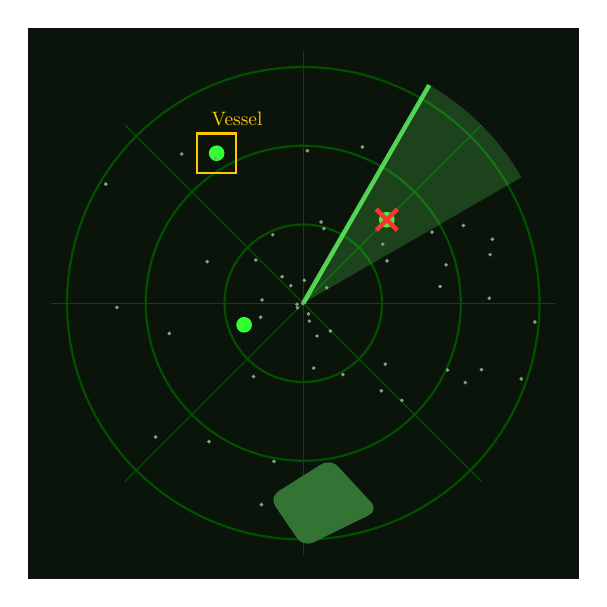
\begin{tikzpicture}[
        ppi/.style={circle, draw=RadarGrid, thick},
        target/.style={circle, fill=RadarTarget, inner sep=2pt, outer sep=1pt},
        clutter/.style={circle, fill=RadarGrid!50, inner sep=0.5pt},
        scale=1.0
    ]
    
    \fill[RadarBackground] (-3.5,-3.5) rectangle (3.5,3.5);
    
    \foreach \r in {1, 2, 3} \draw[ppi] (0,0) circle (\r);
    \foreach \a in {0, 45, ..., 315} \draw[RadarGrid] (0,0) -- (\a:3.2);
    
    \draw[RadarSweep, ultra thick, opacity=0.8] (0,0) -- (60:3.2);
    \fill[RadarSweep, opacity=0.2] (0,0) -- (60:3.2) arc (60:30:3.2) -- cycle;
    
    \node[target] at (45:1.5) {};
    \node[target] at (120:2.2) {};
    \node[target] at (200:0.8) {};
    
    \foreach \i in {1,...,50} {
        \pgfmathsetmacro{\r}{3*rnd}
        \pgfmathsetmacro{\a}{360*rnd}
        \node[clutter] at (\a:\r) {};
    }
    
    \fill[RadarGrid!80, rounded corners] (260:2.5) -- (270:3.1) -- (290:2.8) -- (280:2.0) -- cycle;
    
    \draw[AnnotationBox, thick] (120:2.2) ++(-0.25,-0.25) rectangle ++(0.5,0.5);
    \node[AnnotationBox, above right, scale=0.7] at (120:2.5) {Vessel};
    
    \node[cross out, draw=AnnotationClick, ultra thick, inner sep=3pt] at (45:1.5) {};
    
    \end{tikzpicture}
    }
    \caption{Representative PPI frame showing discrete targets, distributed clutter, and shoreline returns. RADICAL supports both bounding-box and point-click interactions in this visually noisy regime.}
    \label{fig:ppi_example}
\end{figure}

In a PPI plot (Fig.~\ref{fig:ppi_example}), the antenna is at the center and range increases radially. In a range--azimuth plot, the horizontal axis represents azimuth and the vertical axis represents range. Both representations exhibit characteristic artifacts such as beam-width smearing, pulse-length distortion, and side-lobe echoes.

\begin{figure*}[t]
    \centering
    \tikzset{
        radar_crop/.style={
            rectangle, draw=gray, fill=RadarBackground, 
            minimum size=3.5cm, inner sep=0pt
        },
        blob/.style={
            circle, fill=RadarTarget, inner sep=0pt, outer sep=0pt, blur shadow={shadow blur steps=5}
        }
    }

    \begin{subfigure}{0.24\textwidth}
        \centering
        \begin{tikzpicture}
            \node[radar_crop] (bg) {};
            \draw[RadarTarget, line width=4pt, line cap=round] (0,0) arc (45:135:1.0cm);
            \node[text=white, font=\footnotesize, anchor=south] at (bg.south) {A. Beam Smearing};
        \end{tikzpicture}
    \end{subfigure}
    \hfill
    \begin{subfigure}{0.24\textwidth}
        \centering
        \begin{tikzpicture}
            \node[radar_crop] (bg) {};
            \fill[RadarTarget] (-0.3,0) circle (0.5cm);
            \fill[RadarTarget] (0.3,0.1) circle (0.4cm);
            \fill[RadarTarget, opacity=0.5] (0,0.05) circle (0.5cm);
            \node[text=white, font=\footnotesize, anchor=south] at (bg.south) {B. Gain Saturation};
        \end{tikzpicture}
    \end{subfigure}
    \hfill
    \begin{subfigure}{0.24\textwidth}
        \centering
        \begin{tikzpicture}
            \node[radar_crop] (bg) {};
            \foreach \i in {1,...,100} {
                \fill[RadarClutter] (rand*1.5, rand*1.5) circle (0.04cm);
            }
            \fill[RadarTarget] (0.5,0.5) circle (0.2cm);
            \node[text=white, font=\footnotesize, anchor=south] at (bg.south) {C. Rain Clutter};
        \end{tikzpicture}
    \end{subfigure}
    \hfill
    \begin{subfigure}{0.24\textwidth}
        \centering
        \begin{tikzpicture}
            \node[radar_crop] (bg) {};
            \fill[RadarTarget] (0,0) circle (0.3cm);
            \fill[RadarTarget, opacity=0.4] (-0.8,0.1) circle (0.15cm);
            \fill[RadarTarget, opacity=0.4] (0.8,-0.1) circle (0.15cm);
            \node[text=white, font=\footnotesize, anchor=south] at (bg.south) {D. Side Lobes};
        \end{tikzpicture}
    \end{subfigure}

    \caption{Challenges in recreational radar. PPI plots exhibit sensor-specific artifacts such as beam smearing, gain saturation, rain clutter, and side-lobe ghosts that motivate environment-specific overfitting.}
    \label{fig:artifacts}
\end{figure*}

These artifacts highlight why an annotator often needs temporal context and environment-specific behavior from any assisting model.

\subsection{Human-in-the-Loop Annotation}
Human-in-the-loop (HITL) annotation systems often rely on active learning strategies, where a model selects uncertain examples for human labeling. In the radar regime, standard uncertainty metrics such as entropy over class probabilities can be expensive to compute and unreliable in the presence of high, structured noise.

RADICAL instead adopts an implicit-feedback approach. Rather than requiring explicit responses to model queries, the system monitors annotator behavior. The rate and severity of corrections to model suggestions are treated as a direct signal of model usefulness. This idea is related to work in interactive medical-image segmentation, where user corrections drive incremental model refinement~\cite{b3}. If the annotator accepts many consecutive predictions with minimal edits, the model is considered well calibrated for that temporal window.

\subsection{Why Rust?}
Rust is particularly well suited to RADICAL because it combines systems-level control with strong compile-time guarantees about memory and concurrency.

Memory safety without garbage collection is essential when handling large collections of high-resolution radar screenshots. A garbage-collected implementation in Python or Java risks unpredictable pauses that can manifest as visible stutter while scrubbing the timeline. Rust's ownership model and deterministic destruction via RAII (Resource Acquisition Is Initialization) avoid such pauses.

The tool must also run a PyTorch training loop (via C++ bindings) in parallel with a high-frequency rendering loop. Rust's type system and concurrency primitives enable compile-time checking of data races. This ensures that heavy compute threads cannot corrupt GUI state, even under load.

\section{Image Ingestion and Preprocessing}

RADICAL is designed to ingest rasterized radar plots (PNG, JPG, BMP) rather than raw ADC samples. This section describes how these images are transformed into tensors suitable for training a YOLO-style detector.

\subsection{Input Data Format}
RADICAL accepts a directory of sequential images
\(
I = \{i_1, i_2, \dots, i_n\}
\)
that are typically screenshots of a radar display. These images frequently include static user-interface elements such as compass roses, textual readouts, or depth gauges that are irrelevant to detection and can confuse a neural network.

To handle this, the ingestion pipeline includes a configurable cropping region specified at project initialization. The user interactively selects the active radar scope, and the system discards statically overlaid UI regions from all subsequent frames.

\begin{figure}[t]
    \centering
    \begin{tikzpicture}[node distance=0.2cm, auto, >=stealth]
        \tikzset{
            procStep/.style={rectangle, draw, minimum width=1.8cm, minimum height=1.8cm, font=\scriptsize, align=center},
            img/.style={rectangle, fill=RadarBackground, minimum width=1.5cm, minimum height=1.5cm}
        }

        \node[procStep] (s1) {
            \begin{tikzpicture}
                \node[img] {};
                \draw[RadarGrid] (0,0) circle (0.6cm);
                \node[text=RadarGrid, scale=0.5] at (0.5,0.5) {Text};
            \end{tikzpicture}\\
            \textbf{1. Raw}
        };

        \node[procStep, right=of s1] (s2) {
            \begin{tikzpicture}
                \node[img] {};
                \draw[RadarGrid] (0,0) circle (0.7cm);
            \end{tikzpicture}\\
            \textbf{2. Cropped}
        };

        \node[procStep, right=of s2] (s3) {
            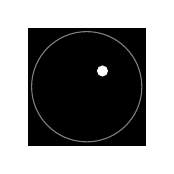
\begin{tikzpicture}
                \node[rectangle, fill=black, minimum width=1.5cm, minimum height=1.5cm] {};
                \draw[gray] (0,0) circle (0.7cm);
                \fill[white] (0.2,0.2) circle (2pt);
            \end{tikzpicture}\\
            \textbf{3. Threshold}
        };

        \node[procStep, right=of s3] (s4) {
            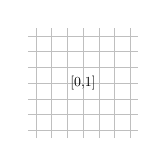
\begin{tikzpicture}
                \draw[step=0.2cm, gray!50, very thin] (-0.7,-0.7) grid (0.7,0.7);
                \node[scale=0.5] at (0,0) {[0,1]};
            \end{tikzpicture}\\
            \textbf{4. Tensor}
        };

        \draw[->, thick] (s1) -- (s2);
        \draw[->, thick] (s2) -- (s3);
        \draw[->, thick] (s3) -- (s4);

    \end{tikzpicture}
    \caption{Ingestion pipeline. The system ingests screenshots, strips UI overlays and color artifacts, and produces a clean intensity tensor for the micro-YOLO network.}
    \label{fig:pipeline}
\end{figure}

\subsection{Tensor Conversion}
To train the YOLO model, each input image is converted into a numerical tensor. The conversion proceeds as follows. First, the image is mapped to a luminance representation. Recreational radar displays are typically monochromatic; the system extracts a luminance channel
\(
L = 0.299R + 0.587G + 0.114B
\),
removing color variations associated with display themes and retaining an intensity map. Second, the cropped scope is resized to the model input size (for example \(416 \times 416\)) using bilinear interpolation. Third, pixel values \(p \in [0, 255]\) are normalized to \(t \in [0, 1]\). The resulting tensor \(T\) is passed to the training and inference threads.

For visualization, RADICAL retains the original high-resolution RGB image. Predictions are rendered as overlays on these originals so that annotators always work with images that faithfully represent the radar display.

\section{System Architecture}

RADICAL is implemented as a single monolithic binary following an event-driven Model--View--Update pattern adapted for heavy asynchronous computation.

\subsection{Safe Concurrency with Rust}
The system uses \texttt{tch-rs} to interface with LibTorch. A central design goal is to ensure that the PyTorch training loop cannot stall the GUI thread. In many Python-based tools, the Global Interpreter Lock (GIL) complicates this separation and often results in frozen UIs during training.

In RADICAL, the deep-learning runtime is encapsulated in a \texttt{TrainingWorker} struct that runs on a dedicated operating-system thread, as depicted in Fig.~\ref{fig:concurrency}. The main thread hosts the GUI and global state, while the worker thread manages training and inference.

\begin{figure}[t]
\centering
\begin{tikzpicture}[node distance=2.0cm, >=stealth, auto]
\tikzstyle{thread} = [rectangle, draw, dashed, inner sep=0.5cm, fill=gray!5, rounded corners]
\tikzstyle{component} = [rectangle, draw, fill=white, drop shadow, text centered, minimum width=2.5cm, minimum height=1cm]
\tikzstyle{data} = [cylinder, shape border rotate=90, draw, aspect=0.25, fill=yellow!20, align=center, minimum width=1.5cm]

\node [thread] (main) {
    \begin{tikzpicture}
        \node[component] (gui) {GUI Loop (60 Hz)};
        \node[component, below=0.5cm of gui] (state) {Global State};
    \end{tikzpicture}
};
\node[above] at (main.north) {\textbf{Main Thread}};

\node [thread, right=3.5cm of main] (worker) {
    \begin{tikzpicture}
        \node[component] (trainer) {YOLO Trainer};
        \node[component, below=0.5cm of trainer] (infer) {Inference Engine};
    \end{tikzpicture}
};
\node[above] at (worker.north) {\textbf{Worker Thread}};

\draw[->, ultra thick, blue] ([yshift=0.5cm]state.east) -- node[above, scale=0.8] {Command Channel} node[below, scale=0.6, text=gray] {(Train, Predict)} ([yshift=0.5cm]infer.west);

\draw[->, ultra thick, red] ([yshift=-0.5cm]infer.west) -- node[above, scale=0.6, text=gray] {(Weights, BBoxes)} node[below, scale=0.8] {Result Channel} ([yshift=-0.5cm]state.east);

\node[data, below=2.5cm of state, xshift=2.5cm] (shmem) {Shared Tensors\\ \texttt{Arc<RwLock>}};

\draw[dashed, thick] (state) -- (shmem);
\draw[dashed, thick] (infer) -- (shmem);

\end{tikzpicture}
\caption{Concurrency architecture. The GUI and global state reside on the main thread, while training and inference execute on a worker thread. Commands and results are exchanged via channels; heavy data are shared via \texttt{Arc<RwLock>} to avoid copying.}
\label{fig:concurrency}
\end{figure}

The main thread sends commands such as \texttt{Command::Train(Batch)} or \texttt{Command::Predict(FrameIndex)} over a command channel and receives completion notifications and predictions over a result channel. Large image tensors are not copied back and forth; instead, an image cache is wrapped in \texttt{Arc<RwLock<ImageCache>}}, allowing concurrent reads from multiple threads while restricting writes to a single ingestion thread.

\subsection{Memory Management}
Long radar sequences can contain thousands of 4K images and easily exceed typical RAM capacities if naively decoded and stored. RADICAL addresses this by memory-mapping raw files from disk and maintaining a Least Recently Used cache of decoded textures. When the user scrubs through the timeline, the system prefetches a window of approximately \(\pm 50\) frames around the current cursor position, decoding them to GPU textures for smooth playback. Frames outside this window are evicted from the cache based on recent access patterns.

\section{Methodology: The Micro-YOLO Strategy}

\subsection{Network Architecture}
The detector in RADICAL is based on a modified YOLO-Tiny architecture. The backbone is reduced to seven convolutional layers, yielding fewer than three million parameters. This small footprint enables training on consumer-grade laptops and allows acceptable performance even when only CPU resources are available.

The architecture is specialized for radar imagery in several ways. The input representation is single-channel grayscale intensity, which focuses the network on geometry and return strength while ignoring display color schemes. Anchor boxes are recomputed using K-means clustering on bounding boxes from a pilot corpus of PPI screenshots, capturing the elongated shapes and smearing patterns characteristic of radar blobs. The network uses two detection scales, such as \(16\times16\) and \(32\times32\) feature maps, which is sufficient because most radar targets occupy small fractions of the scope.

\begin{figure}[t]
    \centering
    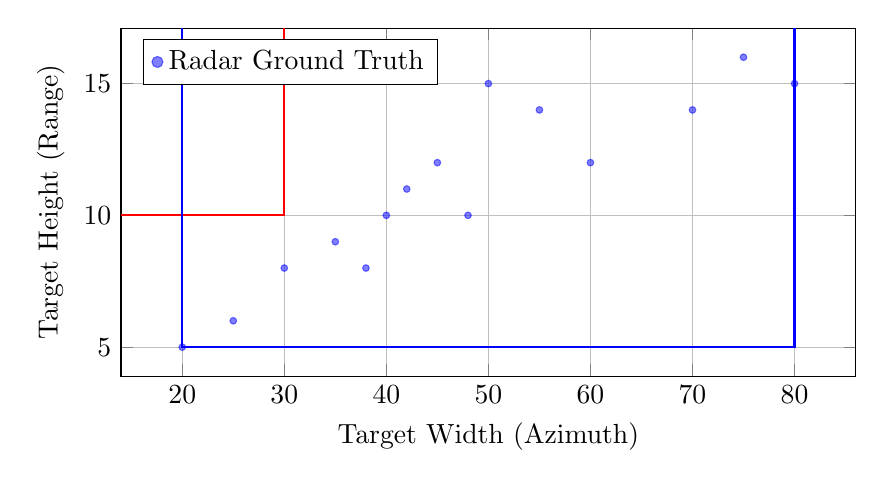
\begin{tikzpicture}
        \begin{axis}[
            width=0.9\linewidth,
            height=6cm,
            xlabel={Target Width (Azimuth)},
            ylabel={Target Height (Range)},
            grid=both,
            scatter/classes={
                a={mark=*,blue, opacity=0.5, scale=0.6},
                b={mark=square*,red, opacity=0.3}
            },
            legend pos=north west
        ]
        
        \addplot[scatter, only marks, scatter src=explicit symbolic]
        coordinates {
            (40, 10) [a] (45, 12) [a] (38, 8) [a] (50, 15) [a] (60, 12) [a]
            (35, 9) [a] (42, 11) [a] (55, 14) [a] (48, 10) [a] (30, 8) [a]
            (20, 5) [a] (25, 6) [a] (80, 15) [a] (70, 14) [a] (75, 16) [a]
        };
        \addlegendentry{Radar Ground Truth}

        \draw[red, thick] (axis cs: 10, 10) rectangle (axis cs: 30, 60);
        \node[red, anchor=south] at (axis cs: 20, 60) {COCO (Tall)};
        
        \draw[blue, thick] (axis cs: 20, 5) rectangle (axis cs: 80, 20);
        \node[blue, anchor=south] at (axis cs: 50, 20) {Custom (Wide)};

        \end{axis}
    \end{tikzpicture}
    \caption{Anchor box distribution. Standard YOLO anchors (red) are ill-suited for radar targets. Custom anchors (blue) derived via K-means match the wide, smeared radar returns.}
    \label{fig:anchors}
\end{figure}

Figure~\ref{fig:anchors} compares typical COCO-style anchors with anchors fitted to radar returns.

\subsection{Loss Function Adaptation}
Standard YOLO loss formulations heavily penalize localization errors, encouraging tight bounding boxes. In radar imagery, precise box boundaries are inherently fuzzy due to blooming and smearing. RADICAL uses a modified loss
\begin{equation}
    L = \lambda_{coord} L_{coord} + \lambda_{obj} L_{obj} + \lambda_{noobj} L_{noobj} + \lambda_{class} L_{class},
\end{equation}
with coefficients tuned to emphasize objectness over exact localization. In particular, the coordinate term weight \(\lambda_{coord}\) is lowered (for example from 5.0 to 2.0) and the objectness weight \(\lambda_{obj}\) is increased (for example from 1.0 to 1.5). The resulting model behaves as a high-recall assistant that proposes coarse regions of interest, which the annotator can refine.

\subsection{Implicit Feedback and Ghost Boxes}

Rather than asking the user to draw all boxes from scratch, RADICAL presents predicted boxes as translucent ``ghost boxes'' that the annotator can accept, reject, or reshape. This interaction is illustrated in Fig.~\ref{fig:ghost_box}. The initial prediction appears as a dashed ghost box with an associated confidence. A single key press confirms the box and converts it into an accepted annotation. When the box is dragged or resized, RADICAL records the resulting correction as both a refined label and an implicit signal that the original prediction was inadequate.

\begin{figure}[t]
    \centering
    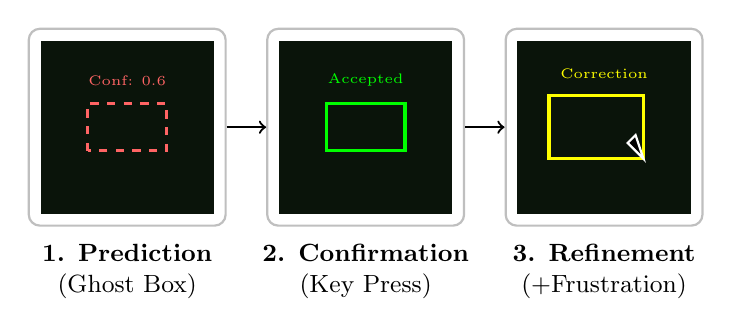
\begin{tikzpicture}[node distance=0.5cm]
        \tikzset{
            state_box/.style={rectangle, draw=gray!50, thick, minimum width=2.5cm, minimum height=2.5cm, rounded corners, fill=white},
            radar_bg/.style={rectangle, fill=RadarBackground, minimum width=2.2cm, minimum height=2.2cm}
        }

        \node[state_box] (s1) {};
        \node[radar_bg] at (s1) {};
        \draw[GhostBox, dashed, very thick] (s1.center) ++(-0.5,-0.3) rectangle ++(1.0,0.6);
        \node[text=GhostBox, font=\tiny, above] at (s1.center |- 0,0.4) {Conf: 0.6};
        \node[below=0.1cm of s1, align=center, font=\small] {\textbf{1. Prediction}\\(Ghost Box)};

        \node[state_box, right=0.5cm of s1] (s2) {};
        \node[radar_bg] at (s2) {};
        \draw[AcceptedBox, very thick] (s2.center) ++(-0.5,-0.3) rectangle ++(1.0,0.6);
        \node[text=AcceptedBox, font=\tiny, above] at (s2.center |- 0,0.4) {Accepted};
        \node[below=0.1cm of s2, align=center, font=\small] {\textbf{2. Confirmation}\\(Key Press)};

        \node[state_box, right=0.5cm of s2] (s3) {};
        \node[radar_bg] at (s3) {};
        \draw[UserBox, very thick] (s3.center) ++(-0.7,-0.4) rectangle ++(1.2,0.8);
        \draw[white, fill=black, thick] (s3.center) ++(0.5,-0.4) -- ++(-0.1,0.3) -- ++(-0.1,-0.1) -- cycle;
        \node[text=UserBox, font=\tiny, above] at (s3.center |- 0,0.5) {Correction};
        \node[below=0.1cm of s3, align=center, font=\small] {\textbf{3. Refinement}\\(+Frustration)};

        \draw[->, thick] (s1) -- (s2);
        \draw[->, thick] (s2) -- (s3);

    \end{tikzpicture}
    \caption{Implicit feedback mechanism. The user sculpts the model's ghost boxes rather than labeling from scratch. The frequency of refinements in State~3 contributes to the Frustration Index.}
    \label{fig:ghost_box}
\end{figure}

\subsection{The Frustration Loop}

The core active-learning mechanism in RADICAL is the frustration loop. Instead of explicitly querying the annotator for labels on selected frames, the system continuously observes how often and how aggressively the annotator edits model suggestions.

Let \(Op(f)\) denote the number of edit operations (clicks, drags, keystrokes) applied to frame \(f\), and let \(N_{\text{targets}}(f)\) denote the number of final objects in that frame. Over a sliding window \(W\) of recent frames, the Frustration Index \(\Phi_t\) at time \(t\) is defined as
\begin{equation}
    \Phi_t = \frac{1}{|W|} \sum_{i=t-W}^{t} \frac{Op(f_i)}{N_{\text{targets}}(f_i) + \epsilon},
\end{equation}
where \(\epsilon\) is a small constant to avoid division by zero. Low values of \(\Phi_t\) indicate that predictions are frequently accepted as-is; high values indicate that the annotator is repeatedly correcting the model.

When \(\Phi_t\) exceeds a threshold \(\tau\) and the training thread is idle, RADICAL triggers a retraining event on the full set of labeled data accumulated so far. New weights are pushed to the inference engine once training converges.

\begin{figure}[t]
    \centering
    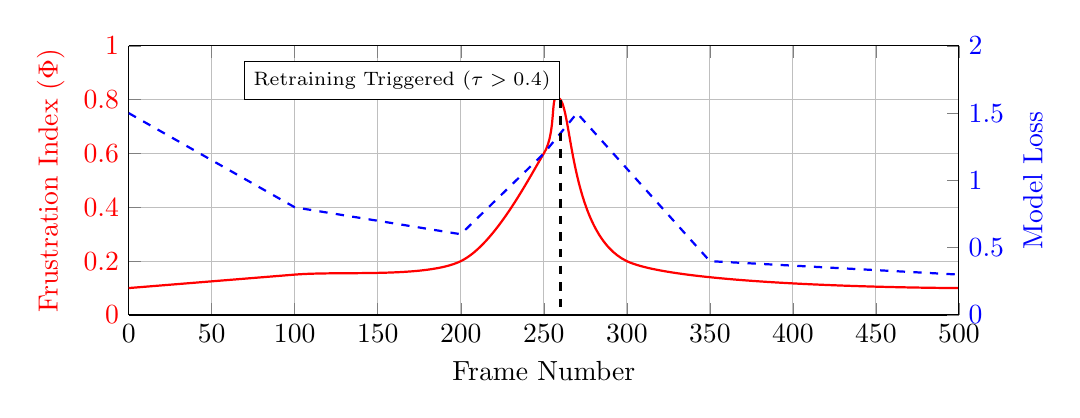
\begin{tikzpicture}
        \begin{axis}[
            width=\linewidth,
            height=5cm,
            axis y line*=left,
            xlabel={Frame Number},
            ylabel={Frustration Index ($\Phi$)},
            ymin=0, ymax=1.0,
            xmin=0, xmax=500,
            grid=major,
            ylabel style={text=red},
            y tick label style={text=red},
        ]
        \addplot[color=red, thick, smooth] coordinates {
            (0, 0.1) (100, 0.15) (200, 0.2) (250, 0.6) (260, 0.8) (300, 0.2) (500, 0.1)
        };
        \node[coordinate] (trigger) at (axis cs:260, 0.8) {};
        \end{axis}

        \begin{axis}[
            width=\linewidth,
            height=5cm,
            axis y line*=right,
            axis x line=none,
            ylabel={Model Loss},
            ymin=0, ymax=2.0,
            xmin=0, xmax=500,
            ylabel style={text=blue},
            y tick label style={text=blue},
        ]
        \addplot[color=blue, thick, dashed] coordinates {
            (0, 1.5) (100, 0.8) (200, 0.6) (250, 1.2) (270, 1.5) (350, 0.4) (500, 0.3)
        };
        \end{axis}
        
        \draw[dashed, thick, black] (trigger) -- (trigger |- 0,0);
        \node[anchor=south east, fill=white, draw=black, font=\scriptsize] at (trigger) {Retraining Triggered ($\tau > 0.4$)};
        
    \end{tikzpicture}
    \caption{Dynamics of the frustration loop. When the environment shifts, prediction quality degrades (blue dashed curve) and user edits spike (red curve), automatically triggering background retraining.}
    \label{fig:frustration}
\end{figure}

\begin{algorithm}[t]
\SetAlgoLined
\KwIn{Stream $S$, threshold $\tau$, window size $W$}
\KwOut{Labeled set $D$}
Initialize $D \leftarrow \emptyset$ and history queue $\leftarrow \emptyset$\;
\While{user is annotating}{
  $F_{\text{curr}} \leftarrow$ current frame\;
  $\hat{y} \leftarrow M(F_{\text{curr}})$\;
  render($F_{\text{curr}}, \hat{y}$)\;
  $(y_{\text{final}}, ops) \leftarrow$ collect user edits\;
  append $(F_{\text{curr}}, y_{\text{final}})$ to $D$\;
  append $ops$ to history\;
  $\Phi \leftarrow$ compute Frustration Index over last $W$ frames\;
  \If{$\Phi > \tau$ and training thread idle}{
     launch background training on $D$\;
  }
  \If{new model weights available}{
     update $M$ with new weights\;
  }
}
\caption{Frustration-driven continual learning loop.}
\end{algorithm}

\section{Experiments and Results}

\subsection{Experimental Dataset}
Experiments were conducted on three sequences of exported images from recreational marine radar units. Sequence~A contains 1500 PPI frames recorded in a busy harbor with a largely stationary own-ship and significant static land clutter. Sequence~B comprises 2200 PPI frames of a vessel underway in open ocean, with high gain noise and multiple moving targets. Sequence~C consists of 1800 range--azimuth frames captured during river transit, where river banks produce strong, continuous clutter lines and targets are challenging to separate from background structure.

\subsection{Annotation Efficiency}
Three graduate students familiar with marine radar were asked to label 500 frames from each sequence under two conditions: a manual baseline using conventional bounding-box tools and an assisted condition using RADICAL. Table~\ref{tab:results} summarizes the annotation time required per 500 frames.

\begin{table}[t]
\caption{Annotation Efficiency Results (Per 500 Frames)}
\label{tab:results}
\centering
\begin{tabular}{@{}llccc@{}}
\toprule
\textbf{Scene} & \textbf{Method} & \textbf{Total Time} & \textbf{Time/Frame} & \textbf{Reduction} \\ \midrule
Harbor & Manual & 28 min & 3.3 s & -- \\
Harbor & Assisted & 14 min & 1.6 s & \textbf{50\%} \\ \midrule
Open Ocean & Manual & 41 min & 4.9 s & -- \\
Open Ocean & Assisted & 26 min & 3.1 s & \textbf{36\%} \\ \midrule
River & Manual & 55 min & 6.6 s & -- \\
River & Assisted & 39 min & 4.6 s & \textbf{29\%} \\ \bottomrule
\end{tabular}
\end{table}

The harbor sequence exhibits the largest time reduction. The scene is structurally stable, and the micro-model quickly learns to ignore static land features while focusing on moving vessels. The river sequence shows smaller gains because changes in bank geometry and strong clutter produce more false positives, which in turn raise the Frustration Index and trigger more frequent retraining.

\subsection{Quantitative Learning Behavior}

To understand how many labeled frames are required before the model becomes useful, an offline study varied the number of labeled frames \(K\) used for training and measured mean Intersection over Union (IoU) on a held-out validation subset. A model was considered useful for annotation assistance once its mean IoU exceeded approximately 0.65.

\begin{figure}[t]
\centering
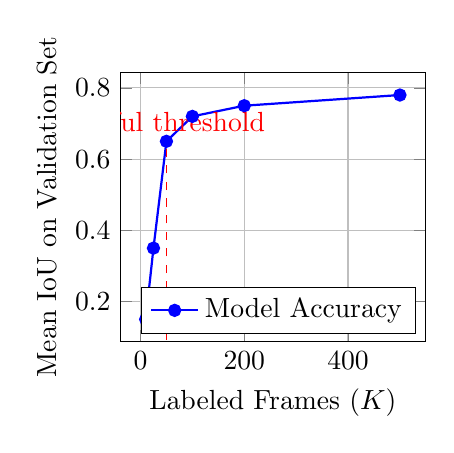
\begin{tikzpicture}
\begin{axis}[
    width=0.45\textwidth,
    height=5cm,
    xlabel={Labeled Frames ($K$)},
    ylabel={Mean IoU on Validation Set},
    grid=major,
    legend pos=south east
]
\addplot[color=blue, mark=*, thick] coordinates {
    (10, 0.15) (25, 0.35) (50, 0.65) (100, 0.72) (200, 0.75) (500, 0.78)
};
\addlegendentry{Model Accuracy}
\draw [red, dashed] (axis cs:50,0) -- (axis cs:50,0.65);
\node [red, anchor=south] at (axis cs:50, 0.65) {Useful threshold};
\end{axis}
\end{tikzpicture}
\caption{Model performance versus number of labeled frames. The micro-model reaches a useful accuracy threshold (mean IoU \(\approx 0.65\)) at approximately 50 labeled frames.}
\label{fig:ablation}
\end{figure}

Figure~\ref{fig:ablation} shows diminishing returns beyond \(K = 100\), supporting the design choice of a small, rapidly trained micro-model rather than a large model requiring thousands of annotated examples.

\subsection{Qualitative Adaptation to Static Clutter}

RADICAL's micro-model quickly internalizes static clutter structure specific to a scene. Figure~\ref{fig:learning_curve} illustrates predictions for a vessel near a jetty at three points in training. Initially, the model produces no meaningful detections. After a cold-start phase, it identifies both the vessel and the jetty as possible targets. After sufficient user feedback, it suppresses the static jetty and retains only the moving vessel as a valid detection.

\begin{figure*}[t]
    \centering
    \tikzset{
        frame/.style={rectangle, draw=gray, fill=RadarBackground, minimum width=4cm, minimum height=4cm},
        jetty/.style={fill=RadarGrid, rounded corners}
    }

    \begin{subfigure}{0.32\textwidth}
        \centering
        \begin{tikzpicture}
            \node[frame] (f1) {};
            \fill[RadarTarget] (0.5, 0.5) circle (0.2cm);
            \fill[jetty] (-1, -1) rectangle (-0.5, 1.5);
            \node[text=white, font=\footnotesize, anchor=north] at (f1.north) {Epoch 0: Initialization};
        \end{tikzpicture}
        \caption{No predictions.}
    \end{subfigure}
    \hfill
    \begin{subfigure}{0.32\textwidth}
        \centering
        \begin{tikzpicture}
            \node[frame] (f2) {};
            \fill[RadarTarget] (0.5, 0.5) circle (0.2cm);
            \fill[jetty] (-1, -1) rectangle (-0.5, 1.5);
            \draw[GhostBox, thick] (0.2, 0.2) rectangle (0.8, 0.8);
            \draw[GhostBox, thick] (-1.1, -0.5) rectangle (-0.4, 0.5);
            \node[GhostBox, font=\tiny] at (-0.7, 0.6) {Vessel?};
            \node[text=white, font=\footnotesize, anchor=north] at (f2.north) {Epoch 50: Cold Start};
        \end{tikzpicture}
        \caption{False positive on jetty.}
    \end{subfigure}
    \hfill
    \begin{subfigure}{0.32\textwidth}
        \centering
        \begin{tikzpicture}
            \node[frame] (f3) {};
            \fill[RadarTarget] (0.5, 0.5) circle (0.2cm);
            \fill[jetty] (-1, -1) rectangle (-0.5, 1.5);
            \draw[AcceptedBox, thick] (0.2, 0.2) rectangle (0.8, 0.8);
            \node[text=white, font=\footnotesize, anchor=north] at (f3.north) {Epoch 150: After Feedback};
        \end{tikzpicture}
        \caption{Jetty suppressed, vessel retained.}
    \end{subfigure}

    \caption{Evolution of on-device learning. Within 150 frames of interaction, the model learns to suppress static jetty clutter specific to this location, a distinction a generic model failed to make.}
    \label{fig:learning_curve}
\end{figure*}

\subsection{System Latency}

A key requirement is that background training must not disrupt GUI responsiveness. The mean frame time of the GUI thread was measured under three conditions. When the system was idle, the frame time was approximately 16.2\,ms (60\,FPS). With CPU-based training running in the background, the frame time increased modestly to 18.5\,ms. With CUDA-enabled training, the frame time was 16.8\,ms. The primary latency spike occurs when the training worker installs a new set of weights, which incurs a one-time cost of roughly 50\,ms corresponding to a small number of dropped frames. Because this update happens infrequently, users reported it as unobtrusive.

\section{Discussion}

\subsection{The Case for Overfitting}
In conventional machine learning, overfitting is treated as a failure mode. For environment-specific annotation assistance, controlled overfitting is a desirable property. The goal is not to produce a detector that generalizes across vessels, harbors, and radar makes, but rather to produce a short-lived model that memorizes idiosyncrasies of a single radar installation and environment. A micro-model that knows, for example, that a particular static shoreline always appears as a bright arc in a given recording can reduce clutter-induced false positives and streamline annotation. RADICAL explicitly embraces this disposable model paradigm.

\subsection{Secure Deployment and Export}

The RADICAL binary does not initiate outbound network connections. All training data, intermediate tensors, and model checkpoints remain on the local device, which can itself be encrypted or otherwise hardened according to operational requirements. The frustration loop provides continual improvement driven solely by local user interactions. These properties make RADICAL suitable for use in regulated environments where radar data cannot be exported to third-party services or cloud platforms.

Once a labeling session is complete, RADICAL can be run in a headless mode that replays the recorded sequence and burns detections into video and metadata streams, as shown in Fig.~\ref{fig:export}. The resulting labeled video and CSV metadata can be archived, shared within secure enclaves, or used to train larger offline models.

\begin{figure}[t]
    \centering
    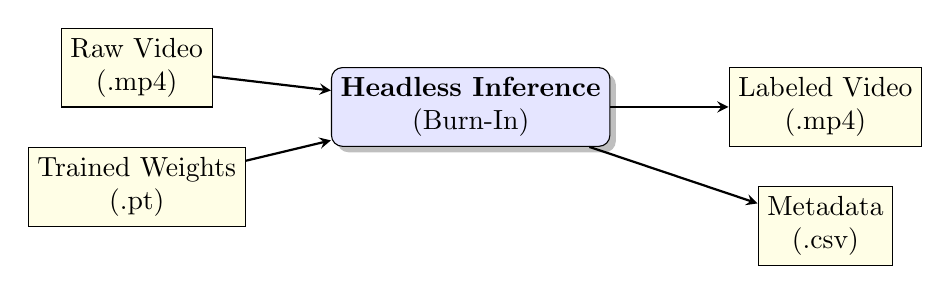
\begin{tikzpicture}[node distance=1.0cm, >=stealth, auto]
        \tikzset{
            file/.style={rectangle, draw, fill=yellow!10, minimum height=1cm, align=center},
            process/.style={rectangle, draw, rounded corners, fill=blue!10, minimum height=1cm, align=center, drop shadow}
        }

        \node[file] (video) {Raw Video\\(.mp4)};
        \node[file, below=0.5cm of video] (weights) {Trained Weights\\(.pt)};
        
        \node[process, right=1.5cm of video, yshift=-0.5cm] (infer) {\textbf{Headless Inference}\\(Burn-In)};
        
        \node[file, right=1.5cm of infer] (out_vid) {Labeled Video\\(.mp4)};
        \node[file, below=0.5cm of out_vid] (out_csv) {Metadata\\(.csv)};

        \draw[->, thick] (video) -- (infer);
        \draw[->, thick] (weights) -- (infer);
        \draw[->, thick] (infer) -- (out_vid);
        \draw[->, thick] (infer) -- (out_csv);

    \end{tikzpicture}
    \caption{Archival workflow. After a session, the tool can run in headless mode to re-play footage and burn the session-specific model's predictions into video and metadata files.}
    \label{fig:export}
\end{figure}

\section{Conclusion}

This work introduced RADICAL, a Rust-based annotation tool for recreational radar imagery that integrates a lightweight YOLO-style detector and a frustration-driven continual learning loop. By training environment-specific micro-models directly on a user's device, RADICAL transforms annotated frames into a feedback signal that accelerates subsequent labeling. Experiments on real radar sequences demonstrate substantial reductions in both annotation time and interaction count, while a carefully engineered concurrency architecture preserves interactivity during background training.

Future work will extend RADICAL beyond 2D radar displays to multimodal settings that include 3D point clouds or camera streams and will explore federated variants of the micro-model strategy in which local models can contribute to shared priors without exposing raw sensor data.

\begin{thebibliography}{00}
\bibitem{b1} Y. Wang, Z. Jiang, X. Gao, et al., ``RodNet: Radar Object Detection using Cross-Modal Supervision,'' \textit{Proc. IEEE/CVF Winter Conf. on Applications of Computer Vision (WACV)}, 2021.
\bibitem{b2} J. Rebut, A. Ouaknine, W. Malik, et al., ``RAW: A Robust and Lightweight End-to-End Radar-Camera Sensor Fusion,'' \textit{IEEE Robotics and Automation Letters}, 2022.
\bibitem{b3} S. Amrehn et al., ``UI-Net: Interactive Artificial Neural Networks for Segmenting Medical Images,'' \textit{Eurographics Workshop on Visual Computing for Biology and Medicine}, 2017.
\bibitem{b4} J. Redmon and A. Farhadi, ``YOLOv3: An Incremental Improvement,'' \textit{arXiv preprint arXiv:1804.02767}, 2018.
\bibitem{b5} B. Settles, ``Active Learning Literature Survey,'' University of Wisconsin--Madison Department of Computer Sciences, Tech. Rep., 2009.
\bibitem{b6} N. Matsunaga et al., ``Rust for Scientific Computing,'' \textit{Journal of Open Source Software}, 2021.
\end{thebibliography}

\end{document}
